\lab{Algorithm}{Invertible Affine Transformations and Linear Systems}{Invertible Affine Transformations and Linear Systems}
\label{lab:ChangeBasis}
\objective{Understand how to apply various affine transformations to a set of vectors and how to solve linear systems.}


\section*{Basis}
A \emph{basis} for a vector space is a linearly independent set of vectors that spans the entire space. Given a basis, it is possible to express every vector in the space as a unique linear combination of the basis vectors (indeed, this property can be taken as the definition for a basis).

Bases themselves are not necessarily unique, however, and it can often be very useful to change the basis representation of vectors, both in theory and practice. Changing bases is an example of an important class of mappings known as \emph{linear transformations}.

In finite dimensional vector spaces like $\mathbb{R}^n$, any linear
transformation can be implemented as a single left matrix multiplication.
In other words, a mapping $T : \mathbb{R}^n \to \mathbb{R}^n$ is linear if and only if there exists an $n \times n$ matrix $A$ such that $T\left(X\right) = AX$ for all vectors $X \in \mathbb{R}^n$. If $A$ is the $n \times n$ matrix representation of a linear transformation and $P$ is an $n \times m$ matrix in $\mathbb{R}^n$, then $AP$ is the matrix of transformed points.

Different linear transformations can be represented by different types of matrices. In this lab we will take vectors in $\mathbb{R}^2$ and apply various linear and affine transformations.

For all the exercises in this lab we will use the following set of points:
\lstinputlisting[style=fromfile]{pts.py}

We have represented each point as a column of the array \li{pts}.
It is also common to represent points as rows. In that case, the transformations described below can still be performed by transposing the arrays in the appropriate places.

\section*{Dilation}
Dilation, or scaling, is a type of linear transformation in which, from a geometrical perspective, points are stretched or compressed.
The matrix representation, $A$, of a dilation is a diagonal matrix. The values on the main diagonal indicate the amount of stretching in their respective directions.

\begin{figure}
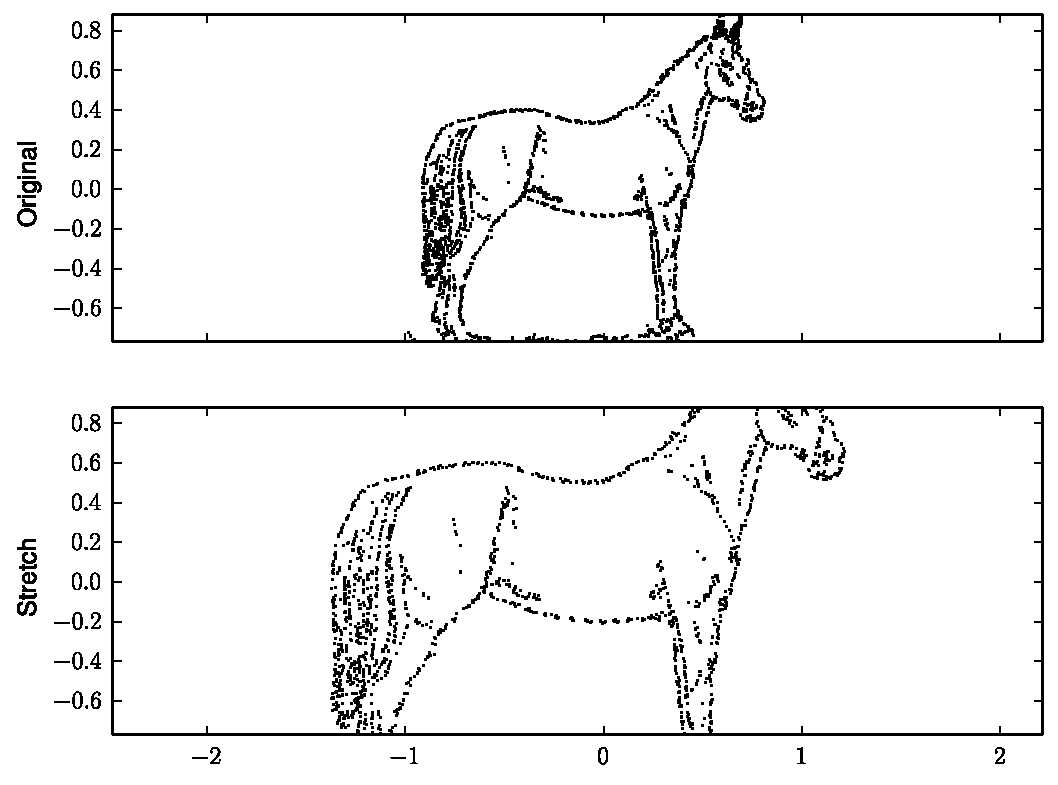
\includegraphics[width=\textwidth]{stretch.pdf}
\caption{An example of a dilation. The top image is the original image and the bottom image is the modified image. The figure was stretched by a factor of $1.5$ in all directions.}
\end{figure}

\begin{problem}
Write a function that accepts an array of points and an array giving the stretching factors in each direction, and returns the dilated points. 

Plot the original points and their image under the transformation. This can be done with the following code:

\lstinputlisting[style=fromfile]{prob1.py}

\end{problem}

\section*{Rotation}
Rotating points around the origin is another type of linear transformation. To perform a rotation of $\theta$ radians counterclockwise, let
\[
A = \begin{pmatrix}
\cos(\theta) & -\sin(\theta) \\
\sin(\theta) & \cos(\theta)
\end{pmatrix}
\]

\begin{figure}
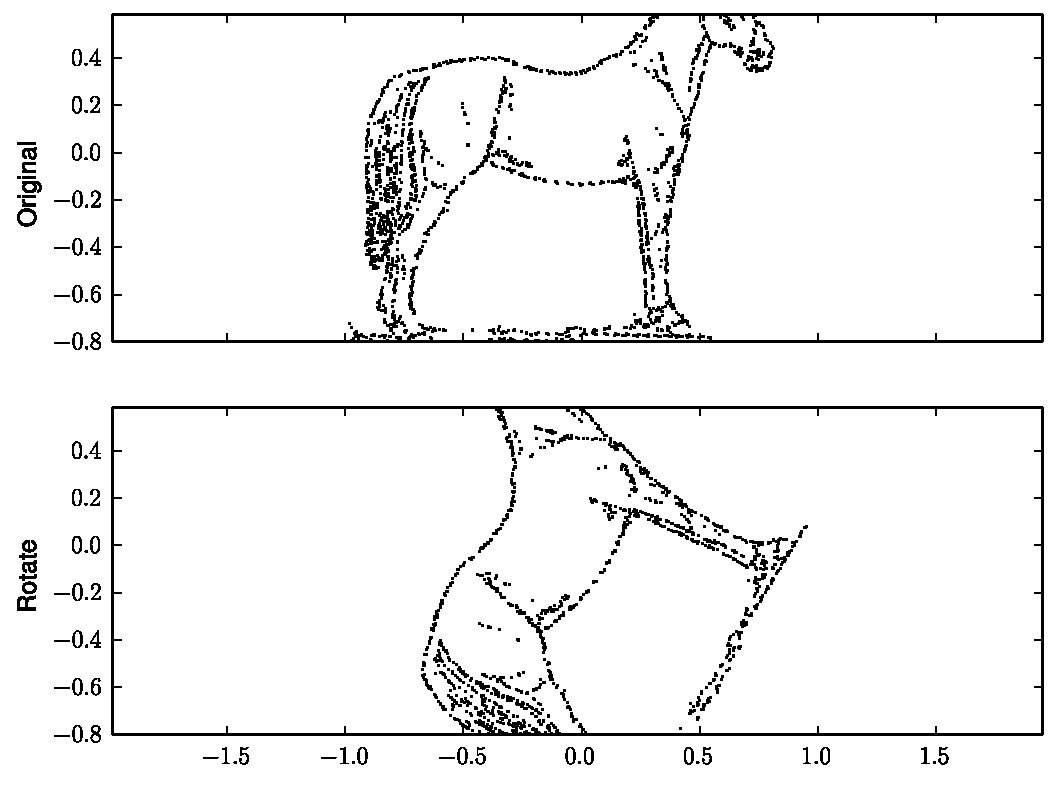
\includegraphics[width=\textwidth]{rotate.pdf}
\caption{An example of a rotation.
The top image is the original and the bottom is the rotated image.
The rotation angle is $\frac{\pi}{3}$.}
\label{basis:rotate}
\end{figure}

\begin{problem}
Write a function that accepts an array of points and the angle of rotation (in radians). Have it return the rotated points.
Plot the original points and their image under the transformation.
\end{problem}

\section*{Shear}

\begin{figure}
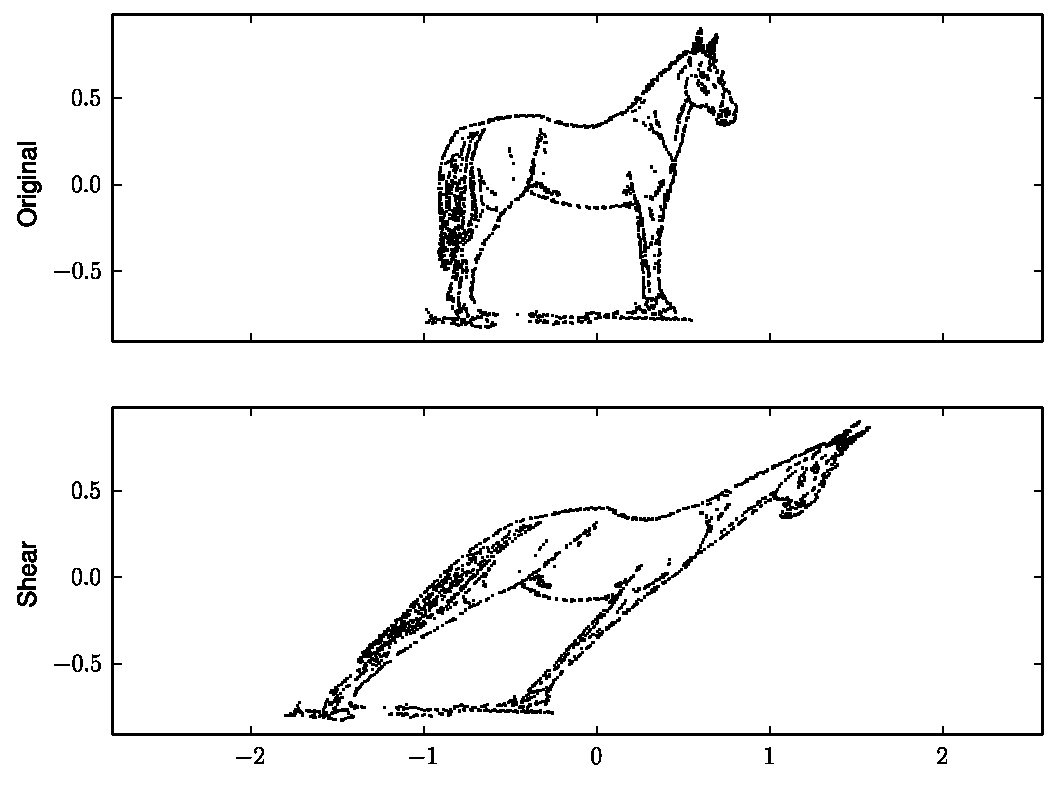
\includegraphics[width=\textwidth]{shear.pdf}
\caption{An example of a shear.
The top image is the original and the bottom is the sheared image.}
\label{basis:shear}
\end{figure}

A shear is a linear transformation that displaces a vector in a fixed direction. In $\mathbb{R}^2$, a shear can either be horizontal or vertical, and has one of the two following forms, respectively:

\[
A = \begin{pmatrix}
1 & c \\
0 & 1
\end{pmatrix}
\]

\[
A = \begin{pmatrix}
1 & 0 \\
c & 1
\end{pmatrix},
\]

where $c$ indicates the amount of displacement.  

Note that these shearing matrices are instances of a type III elementary matrix. Horizontal shears leave the y-coordinates fixed, while vertical shears leave the x-coordinate fixed. 

\begin{comment}
In physics, shears are examples of what are known as Galilean Transformations, and are used to switch between reference frames that differ only by constant relative motion.
\end{comment}

\begin{problem}
Write a function that accepts an array of points, a floating point argument that indicates the shearing amount, and an integer argument
that indicates the direction of shearing (0 for horizontal, 1 for vertical). Have it return the sheared points.
Plot the original points and their image under the transformation.
\end{problem}

\section*{Reflection}

\begin{figure}
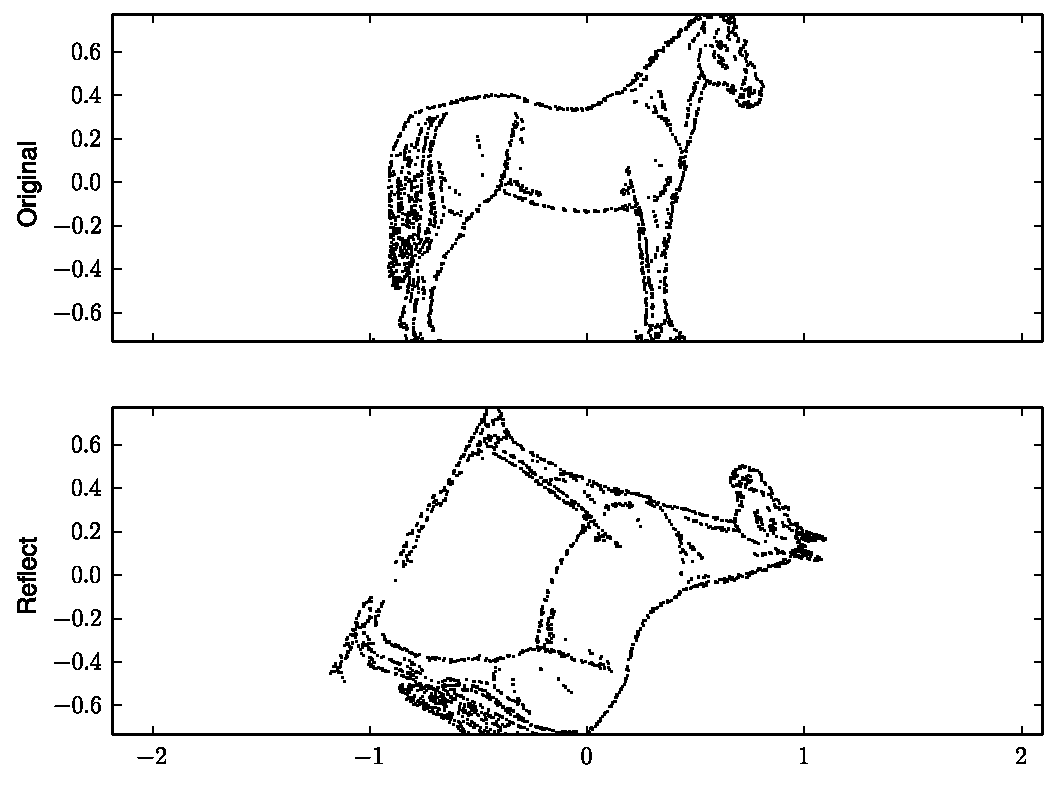
\includegraphics[width=\textwidth]{reflect.pdf}
\caption{An example of a reflection. The top image is the original and the bottom is the image after being reflected about the line $y = \sqrt{3}x$.}
\label{basis:reflect}
\end{figure}

Reflection about a line (or in higher-dimensional spaces, a hyperplane) can also be accomplished by a linear transformation. Such a transformation is called a \emph{Householder Transformation}, and the general form of the matrix representation in
$\mathbb{R}^2$ is

\[
A = \frac{1}{l_1^2 + l_2^2}
\begin{pmatrix}
l_1^2 - l_2^2 & 2l_1l_2 \\
2l_1l_2 & l_2^2 - l_1^2
\end{pmatrix},
\]

where $(l_1, l_2)$ is a vector in the direction of the axis of reflection. In the simple case where the axis of reflection is the line $y=x$, the matrix is just a Type I elementary matrix. See Figure \ref{basis:reflection} for an example.

\begin{problem}
Write a function that accepts an array of points and an array giving the axis of reflection (in the notation above, this argument is $(l_1, l_2)$. Have it return the reflected points.
Plot the original points and their image under the transformation.
\end{problem}

\section*{Translation}

\begin{figure}
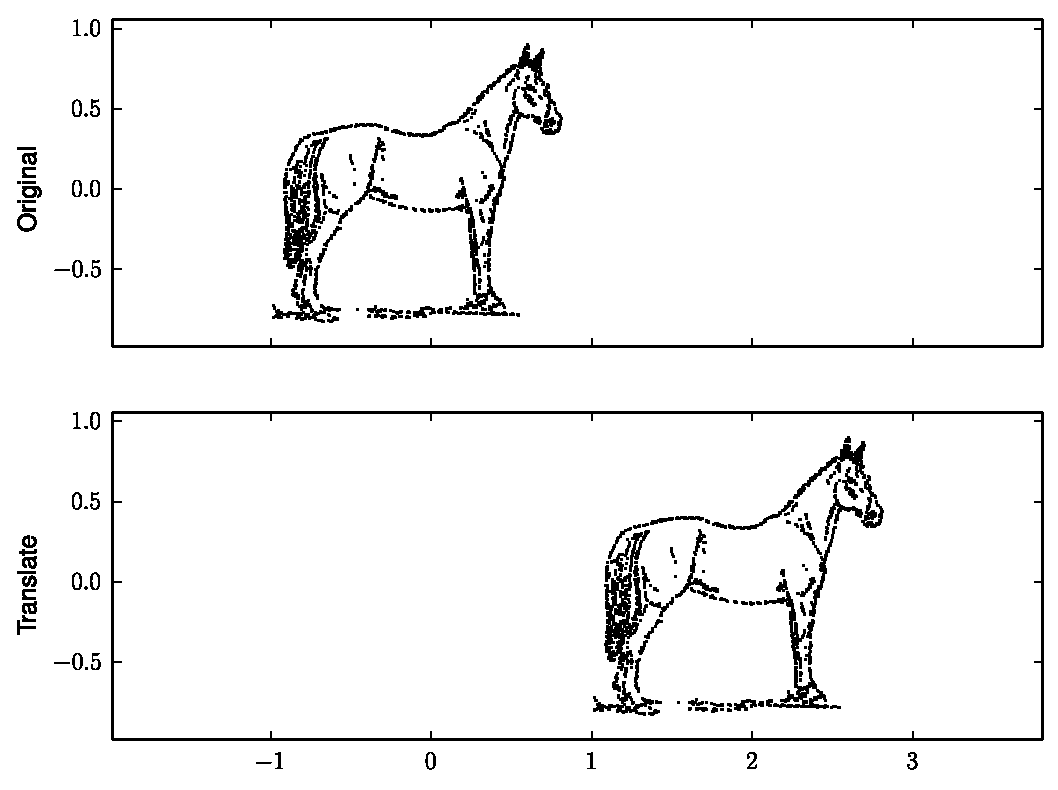
\includegraphics[width=\textwidth]{translate.pdf}
\caption{
An example of a translation.
The top image is the original and the bottom is the translated image.}
\label{basis:translate}
\end{figure}

Translations are not linear transformations, but they can easily be performed with array operations. Together, with linear transformations, they make up the broader class of transformations called
``affine transformations." These are transformations of the form $T: \mathbb{R}^n \to \mathbb{R}^n$, $T(X) = AX + b$ where $A$ is an $n\times n$ matrix and $b \in \mathbb{R}^n$. Affine transformations include all compositions of scalings, rotations, and translations.


Let $b$ be a vector that represents the desired translation.
In order to shift a set of points, you add to the row how much you would like it to shift in that direction. Thus, to shift the set of points up by 2, simply add \li{b = np.array([[0], [2]])}. This particular shape for $b$ allows for proper array broadcasting.
See Figure \ref{basis:translation} for an example.

\begin{problem}
Write a function that takes an array of points and an array indicating how much to shift them in each direction. The function should return the translated points.
Plot the original points and their image under the transformation.
\end{problem}

\section*{Compositions of Transformations}

\begin{figure}
\centering
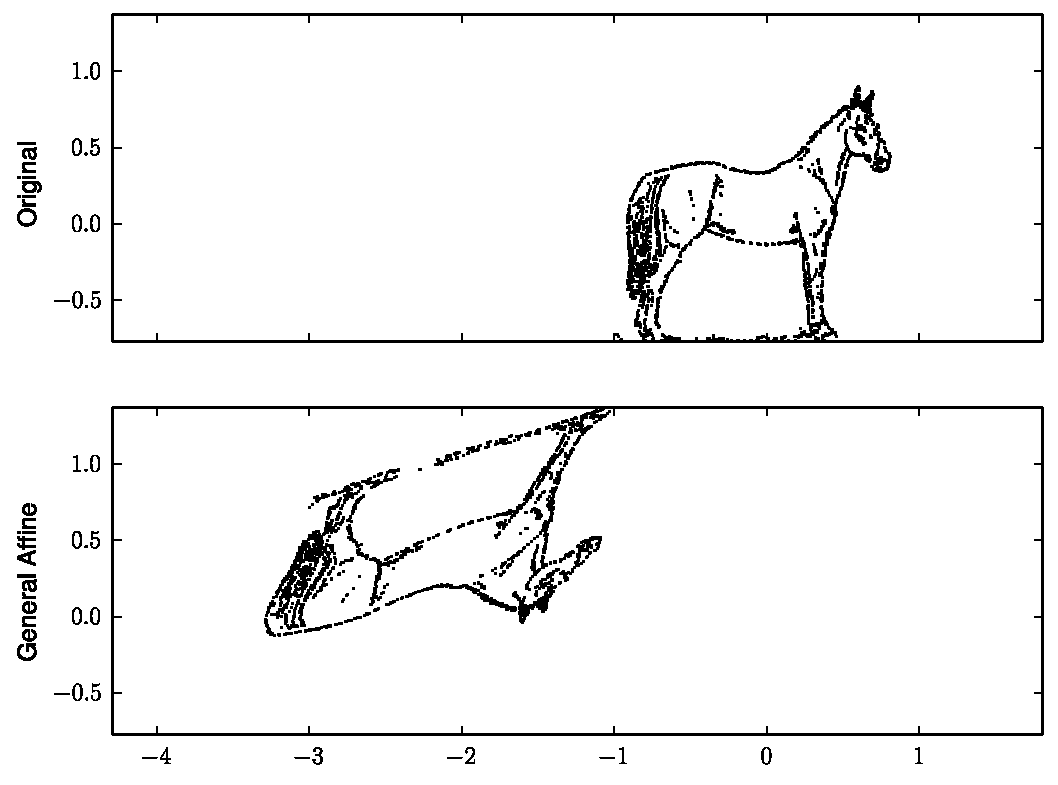
\includegraphics[width=\textwidth]{combo.pdf}
\caption{
A composition of affine transformations: shear, reflection, and translation.}
\label{basis:combo}
\end{figure}

All the various transformations we have discussed can be combined into a single affine transformation through function composition.
For example, if you want to apply a shear and then a reflection, you can represent the shear as a matrix $S$ and the reflection as a matrix $R$. The combined transformation is then $RS$. The image of $X$ under both transformations and then a translation that moves the origin to point $P$ would be $RSX+P$. An example of this is shown in Figure \ref{basis:combo}.

\begin{problem}
We can use affine transforms to track the trajectory of a particle $p_1$ that rotates about another particle $p_2$ at a constant angular speed $\omega$ (a positive value means counterclockwise rotation), while $p_2$ moves in a particular direction at a constant speed $v$. 

Suppose that $p_2$ has a starting position at the origin and moves in the direction of the vector $(1, 1)$, and suppose that $p_1$ has a starting position at the point $(0,1)$. Write a function that takes three parameters giving the time, angular velocity, and directional speed, respectively, and returns the position of $p_1$ at the given  time.

Visualize a trajectory by plotting the position of the particle at each time (in seconds) in the array \li{times = numpy.arange(0,10,.1)} for an angular velocity $\pi$ radians per second and a directional speed of 3 meters per second (assume the plot is on a meters scale).
\end{problem}

\section*{Linear systems}
Matrices are powerful for many reasons. Once such reason is that they can be used to represent linear systems of equations. This next section focuses on better ways to solve systems of linear equations by manipulating matrices.

\section*{Elementry row operations}
In linear algebra there are three elementary row operations on matrices: switching two rows, multiplying a row by a constant, and adding a multiple of one row to another row. Each of these operations can, in theory, be done through left multiplication by the appropriate elementary matrix. This approach is \emph{extremely} slow in practice.
It is much faster to perform these operations directly by modifying only the portions of an array that change as a result of the row operation.


The following code shows how these modifications can be made in-place to an array.

\lstinputlisting[style=fromfile]{row_opers.py}

\section*{Programming Row Reduction}
Solving a linear system can be done most efficiently by using elementary row operations to reduce a matrix to \emph{row echelon form} (REF), as opposed to \emph{reduced row echelon form} (RREF).
Consider the following matrix:

\[
\begin{pmatrix}
4&5&6&3 \\
2&4&6&4 \\
7&8&0&5
\end{pmatrix}
\]

Using elementary row operations, we can reduce $A$ to REF as follows:

\begin{lstlisting}
>>> import numpy as np
>>> A = np.array([[4., 5., 6., 3.],[2., 4., 6., 4.],[7., 8., 0., 5.]])
array([[ 4.,  5.,  6.,  3.],
       [ 2.,  4.,  6.,  4.],
       [ 7.,  8.,  0.,  5.]])
>>> A[1] -= (A[1,0]/A[0,0]) * A[0]
>>> A[2] -= (A[2,0]/A[0,0]) * A[0]
>>> A[2,1:] -= (A[2,1]/A[1,1]) * A[1,1:]
>>> A
array([[ 4. ,  5. ,  6. ,  3. ],
       [ 0. ,  1.5,  3. ,  2.5],
       [ 0. ,  0. , -9. ,  1. ]])
\end{lstlisting}

The additional requirement is often added that the first nonzero entry of each row be 1. Do not worry about that requirement here.
Notice that in our third row operation we were able to operate on only a portion of the third row because we knew that the first value would still be 0. In this case it made little difference, but it is good to watch for things like this because they can save a great deal of time when working with larger matrices.

A brief discussion of some potential pitfalls is in order.
Round-off error can lead to serious numerical issues. Consider the
following variation on the above example.

\begin{lstlisting}
>>> A = np.array([[4., 5., 6., 3.],[2., 2.5, 6., 4.],[7., 8., 0., 5.]])
array([[ 4.,  5.,  6.,  3.],
       [ 2.,  2.5,  6.,  4.],
       [ 7.,  8.,  0.,  5.]])
>>> A[1] -= (A[1,0]/A[0,0]) * A[0]
>>> A[2] -= (A[2,0]/A[0,0]) * A[0]
\end{lstlisting}

If we work this out by hand, we should currently have

\[
\begin{pmatrix}
4&5&6&3 \\
0&0&3&2.5 \\
0&-7.5&-10.5&-.25
\end{pmatrix}.
\]

All that is left is to swap the second and third rows, and the matrix is in row echelon form. However, suppose that due to numerical round-off error, the machine instead computes:

\[
\begin{pmatrix}
4&5&6&3 \\
0&10^{-15}&3&2.5 \\
0&-7.5&-10.5&-.25
\end{pmatrix}.
\]

The algorithm would then attempt to pivot on the \li{A[1,1]} entry:

\begin{lstlisting}
>>> A[2,1:] -= (A[2,1]/A[1,1]) * A[1,1:]
>>> A
array([[ 4. ,  5.0e+00 , 6.00e+00 ,  3.000e-00 ],
       [ 0. ,  1.0e-14 , 3.00e+00 ,  2.500e-00 ],
       [ 0. ,  0.0e+00 , 2.25e+14 ,  1.875e+14 ]])
\end{lstlisting}

The round-off error in the \li{A[1,1]} entry has affected the third
row, and the matrix is now much different than our first calculation. In larger matrices, such an error could potentially propagate through many steps in the calculation, resulting in garbage output.

This example also illustrates another issue to be aware of. Even if there were no round-off error in the \li{A[1,1]} entry, a naive implementation of the algorithm might still attempt to pivot on that entry, which would result in division by zero. As noted above, we would first need to swap rows 2 and 3 in order to proceed. Dealing with leading zeros by permuting the rows is another consideration when designing a fool-proof REF solver.

\begin{problem}
\label{prob:REF}
Write a Python function which takes a matrix and reduces it to REF.
Assume that the matrix is invertible and ignore the possibility that a zero may appear on the main diagonal during row reduction. You are not
responsible for dealing with potential round-off errors.
\end{problem}

\section*{LU Decomposition}
LU Decomposition refers to a process for factoring a square matrix into the product of a lower triangular matrix and an upper triangular matrix. Such a factorization exists only for certain classes of matrices. In the case of an invertible $n \times n$ matrix $A$, the LU decomposition exists if and only if all of the leading principle minors are non-zero (that is, all of the submatrices \li{A[:k,:k]} for $k = 1,\ldots,n-1$ are invertible). Even in this case, however, it may still be necessary to permute the rows of the matrix in order to prevent zeros from appearing on the main diagonal. Thus, row swap operations are, in general, necessary for the LU decomposition.

Using row reduction we can reduce the matrix $A$ to upper triangular form. Say this can be done in $k$ row operations.
Let $U$ be the upper triangular form of $A$, so we have:

\[
U = E_k \dots E_2 E_1 A.
\]

Since the elementary matrices are invertible, we also have

\[
(E_k \dots E_2 E_1)^{-1} U =  A.
\]

Then we define $L$ to be

\[
L = (E_k \dots E_2 E_1)^{-1}
\]

which is the same as

\[
L = E_1^{-1} E_2^{-1} \dots E_k^{-1}
\]

In either case we have $L U = A$.

The inverses of elementary matrices are also elementary matrices. Thus, $L$ can be computed by applying a series of simple operations to an identity matrix.
Note when we are only doing type 3 row operations, each of the operations represented by right multiplication by these inverse matrices results in the change of a single entry in $L$.

In practice, the LU decomposition of an array $A$ can be computed like this:

\begin{itemize}
\item Make a copy, $U$, of $A$.
\item Make an identity matrix $L$ that is the same shape as $A$.
\item Iterate through the entries below the diagonal of $U$.

Now for each entry below the main diagonal of $U$ do the following:
	\begin{itemize}
	\item Set the corresponding entry of $L$ to the quotient of the current entry of $U$ and the entry of the main diagonal of $U$ located above the current entry.
	\item Perform the type 3 row operation to set the current entry of $U$ to 0.
		Remember to avoid computation involving columns that have already been processed.
	\end{itemize}
\item Return $L$ and $U$
\end{itemize}

In this case, we have ignored the possibility that a 0 may appear along the main diagonal during computation. A full implementation of the LU decomposition would have to account for this possibility as well by swapping rows appropriately.

\section*{Why This Matters}
The LU decomposition is more efficient for solving linear systems than traditional row reduction and also allows for quick computation of inverses and determinants. For very large matrices, the LU decomposition can be performed without using any extra space as follows: $L$ is stored above the main diagonal of the array and $U$ is  stored below it.
Note there is no need to store the main diagonal of $L$ since all its entries are ones.

\begin{problem}
\label{prob:LU}
Write a function takes in an $n\times n$ matrix, performs the LU decomposition, and returns $L$ and $U$.
To verify that it works, multiply $L$ and $U$ together and compare to $A$.
Assume that the matrix is invertible and ignore the possibility that a zero may appear on the main diagonal during row reduction.

Write another version of the function that modifies its input in place, storing $L$ below the main diagonal and $U$ in the rest of the array.
\end{problem}

As noted earlier, in general one needs to consider row-swapping when
calculating the LU decomposition. This means that it is not always possible to simply have

\[
A = LU,
\]
but rather

\[
PA = LU,
\]

where $P$ is a permutation matrix representing the necessary row-swaps. Given such a decomposition, we can solve the linear system $Ax = b$ by
first solving $Ly = Pb$ and then $Ux = y$. Since $L$ and $U$ are triangular, these systems can be solved easily with backward and forward substitution. We can use this technique to calculate $A^{-1}$ by solving the matrix equation $LUX = P$ column-by-column. Finally, we can calculate the determinant of $A$ via the formula

\[
\det(A) = (-1)^S\left(\displaystyle\prod_{i=1}^nu_{ii}\right),
\]

where $S$ is the number of row-swaps.

SciPy includes a complete implementation of the LU decomposition in the \li{linalg} module. Furthermore, several other methods in the \li{linalg} module are based on the LU decomposition, including \li{linalg.solve}, \li{linalg.inv}, and \li{linalg.det}.

\begin{problem}
\label{prob:Solve}
Suppose there is a need to solve the system $Ax = b$ for fixed $A$ and many different values of $b$. It would be unwise to perform row-reduction for every single new value of $b$, and the LU decomposition helps us avoid this and save time.

Create a random $1000 \times 1000$ array $A$, and a random $1000 \times 500$ array $B$. Use the \li{scipy.linalg.lu_factor} function to compute the LU factorization of $A$. Then use the \li{scipy.linalg.lu_solve} function to solve the system $AX = B$, and time this operation. 

Now use the \li{scipy.linalg.inv} function to compute the inverse of $A$, and then use it to solve the system $AX = B$. Again time the operation. 

\end{problem}

%\begin{problem}
%\label{prob:lusolve}
%Write a function that takes the LU decomposition computed by the second function you made in Problem \ref{prob:LU} and another array representing the right hand side of a linear system and modifies the second array in place so that it represents the solution to the linear system.
%No changes to the array storing the LU decomposition are necessary.
%\end{problem}
%

\begin{problem}
\label{prob:det}
Write a function which takes as input a square matrix $A$ and uses \li{linalg.lu_factor} to find the determinant of $A$. Note that \li{linalg.lu_factor} returns a square array \li{lu} that contains $U$ in its upper triangle, as well as an array \li{piv} that represents the 
permutation matrix $P$. Use \li{piv} to compute the number of row swaps, and use the \li{diagonal} method on \li{lu} to compute the product of the diagonal terms, as needed in the formula for the determinant.

Hint: if the $i^{th}$ entry of \li{piv} does not equal $i$, this means that a row swap occurred.
\end{problem}

\section*{The Cholesky Decomposition (Optional)}

Under certain conditions, the Cholesky decomposition offers a more efficient alternative to the LU decomposition.
It requires half the number of calculations and half the memory that the standard LU decomposition needs.
Furthermore, it is a \emph{numerically stable} decomposition, which means that round-off and truncation errors are kept suitably under control, rather than growing and propagating throughout the computation.
Because of the efficiency and numerical stability, Cholesky decomposition is used in solving least squares, optimization, and state estimation problems.
The Cholesky decomposition, however, is only applicable to Hermitian (for real matrices, this means symmetric) positive definite matrices.
It can be thought of as the matrix equivalent to taking the square root of a positive real number.

The Cholesky decomposition of a $A$ is a lower-triangular matrix, $L$, such that

\begin{equation*}
 A = LL^*
\end{equation*}

Where $L^*$ is the conjugate transpose of $L$.
For real valued matrices, this is equivalent to $L^T$.

The entries of $L$ are calculated as follows.

\begin{align*}
&L_{i,j} = \frac{1}{L_{j,j}}\left(A_{i,j} -\sum_{k=1}^{j-1}{L_{i,k}L_{j,k}^*}\right) \mbox{ for $i>j$} \\ \\
&L_{i,i} = \sqrt{A_{i,i} - \sum_{k=1}^{i-1}{L_{i,k}L_{i,k}^*}}
\end{align*}

where $L^*$ denotes the conjugate transpose of $L$.

Notice that in this computation, current calculation will depend on previous calculations. To calculate $L$ properly, you must start in the upper left corner and iterate down.

Note: when testing positive definite systems, an easy way to generate a random symmetric positive definite matrix is by generating a random array \li{A} and then computing \li{A.dot(A.T)}.

\begin{problem}
Write your own implementation of the Cholesky decomposition.
Test it using a random symmetric matrix (build a random square matrix $A$, then $A^TA$ will be positive definite).
Check the output of your function to ensure that it is functioning properly.
\end{problem}

%\begin{problem}
%Modify your previous answer so that it computes the Cholesky decomposition by modifying the array in place.
%Make sure you set the portion of the array above the main diagonal to 0.
%Then write a function that takes this reduced form of the array and uses it to solve a linear system by back substitution.
%This should be nearly the same as Problem \ref{prob:lusolve}.
%\end{problem}

The linalg module of SciPy also includes a Cholesky decomposition that should be much faster than the one you just implemented. It works much like the LU decomposition, providing the methods \li{cho_factor} and \li{cho_solve}.

\begin{problem}
Repeat the steps in problem \ref{prob:loopSolve}, this time using the
Cholesky decomposition. Make sure the input matrix to be factored is
positive definite.
\end{problem} 
